\subsection{Generating Unit-Level Assertions} \label{Sec:unitLevelAssertion}
Our approach targets postcondition assertions which are used to examine the expected behaviour of a given function after it is executed in a unit test case.
Through analyzing a given DOM-based test case, we generate unit-level assertions in the following three categories: (1) assertions, which are directly related to a given DOM-based assertion, (2) assertions, which are indirectly affected by a given DOM-based assertion, and (3) assertions that have direct impact on important DOM elements which are not checked by the existing DOM-based assertions. In the following we explain each category in details.
\subsubsection{Explicit Assertions} \label{Sec:explicitAssertions}
After collecting all the statements, that are relevant to a given DOM-based assertion, we extract accessible entities from these statements.
Accessible entities include (1) the function's returned value, (2) the used global variables in that function, (3) the object's property where the object is accessible in the outer scope of the function, and/or (4) the accessed DOM element in that function. Dynamic backward slice of a DOM-based assertion helps to (1) track all statements that contribute to the checked result and as such identify those entities that might have influenced the checked property value of the DOM element, and (2) eliminate unrelated entities which are not involved in the computation that leads to the update performed on the checked DOM element.

Since our dynamic slice is extracted from the program run, we can track all concrete values associated with accessible entities.
During the run of a test case, there might be different instances where a given statement is executed. Different execution instances can lead to different behaviour. Since we are employing dynamic slicing, an instance that leads to the required behaviour, which is verified through the DOM-based assertion, is on the backward slice. Given that the manually-written expected value, that is checked against the DOM's property is valid, the concrete values of related entities in the backward slice are potentially correct unless there exists a masked fault which is concealed in the chain of computations and thus does not propagate to the checked state of the DOM element. We conjecture that fault masking rarely happens in \javascript web applications as it is more prevalent in programs with many small expressions whose results are stored in several intermediate values (we further discuss this in the evaluation section). Therefore, concrete value of an entity in the backward slice can potentially be used as the expected value of the entity in unit-level assertions to test the current version of the application.
%We compare the value of the entity immediately after the relevant statement is executed in the backward slice with the entity's value before the function exits. If value of the entity remains the same, we use it towards the expected value in the unit-level assertion.  
%However, if the entity pertaining to a DOM change is reassigned in the code after the DOM gets updated and before the function exits, then the concrete value of the entity can be used for the purpose of regression testing unless the tester provides the proper expected value.
\subsubsection{Implicit Assertions} \label{Sec:implicitAssertions}
We gather all the statements that explicitly affect the computations relevant to a given DOM-based assertion. While assertions inferred from such statements are inherently important, we further need to consider entities that are implicitly influenced by the checked DOM element in the manually-written test suite. For this purpose we apply a dynamic forward slice on the statements collected from a backward slice of a DOM-based assertion.
%\begin{mydef}[Forward Slicing]
%\label{def:forwardSlicing} 
%A forward slice of a program with respect to a statement $st$ at program point $p$ and set of program variables $V$ consists of all statements and predicates in the program that are affected by the value of variables in $V$ at $p$.
%\end{mydef}
A forward slice with respect to a statement $st$,
indicates how subsequently an operand at $st$ is being used. This can help the tester to ensure that $st$ establishes the expected outcome of the computations assumed by later statements. 
%Given the importance of statements involved in code-level computations of a DOM-based assertion, using forward slice is useful to check that there are no unforeseen effects on the application's behavior by a modification to such statements. 

\begin{figure}[!t]
  \centering
  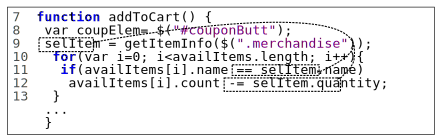
\includegraphics[width=1\hsize]{fig/forwardSlicingExample}
   \vspace{-0.2in} 
  \mycaption{Forward Slicing to obtain implicit assertions.}
  \label{Fig:forwardSlicingExample}
 % \vspace{-0.1in} 
\end{figure}

Dynamic forward slice is performed on the subset of code statements which is previously instrumented as explained in \secref{domToCode}. 
\textsc{GetFWSlice} in line 17 of the algorithm computes forward slice on the variable operands of a statement in the backward slice.
The process of forward slicing is similar to the backward slicing technique discussed earlier (\secref{domToCode}). The slicing criterion of the forward slice module is either a variable, object's property, or an accessed DOM property extracted from the statements in a backward slice segments of the code. The accessible entities (\textsc{Accessibles} in line 24), which have been set within the collected forward slice statements establish the implicit assertions.
$implicitAsstn$ in line 24 of \algref{algorithm} contains the inferred implicit assertions.
\figref{forwardSlicingExample} shows the relevant parts of the code obtained by performing forward slicing on the running example. 
As shown in the figure, the properties of object \code{selItem} are set in line 16, that is recorded during the backward slice process. Given line 16 as the forward slice criteria, we mark \code{availItems.count} (line 19) as an implicit assertion.        
\input{potentialAssertions}
 